\section{License}

    Copyright (c)  2024 Leandro Ebner. \\
    Permission is granted to copy, distribute and/or modify this document under the terms of the GNU Free Documentation License, Version 1.3 or any later version published by the Free Software Foundation; with no Invariant Sections, no Front-Cover Texts, and no Back-Cover Texts. A copy of the license can be found here:
    \href{https://www.gnu.org/licenses/fdl-1.3.txt}{https://www.gnu.org/licenses/fdl-1.3.txt}.

    \begin{figure}[h!]
    
\includegraphics{contents/figures/gfdl-logo.png}
    \end{figure}
    
\section{Introduction}

    This document will serve as a comprehensive guide through the entire power distribution and wiring system of our rover. It meticulously details all relevant safety measures designed to minimize the likelihood of hazards or environmental damage. By following these guidelines, we aim to ensure that our work adheres to the highest safety standards. 

    \vspace{5mm}

    In addition to outlining essential safety protocols, this guide sets forth the minimum standards for both material and personal safety. These standards apply not only during the construction phase but also throughout the actual operation of all electronic components. To enhance understanding and clarity, we have included several schematics, data sheets, and detailed calculations. These resources are designed to provide a thorough illustration of the rover's internal architecture and functionality, making the document as informative and accessible as possible.

    \begin{table}[b]
        \centering
        \begin{tabular}{|c|c|c|c|} \hline 
             Revision&  Date submitted& Summary of changes  &Authored\\ \hline 
             v1.0.0&  16.06.2024& Initial release  &Leandro Ebner\\ \hline
        \end{tabular}
    \end{table}
    \clearpage

\section{Hazardous Material List}

    \clearpage
    
\section{Power Architecture}

    The rover's power architecture is divided into two separate power systems. This approach ensures galvanic isolation between the power and logic components, which is necessary to eliminate any possible wiring configuration in which a so-called "ground loop" could form. The underlying problem is based on the fact that there exists an interface and thus an electrical connection between the individual components. While the communication between power and logic components is implemented by establishing a physical connection between their corresponding GPIO pins and reading different voltage levels, there must be a precise reference voltage available. Generally speaking, this is done by using a common ground. Hence, the most basic form to utilize that common ground connection is to form a "star ground." If there are multiple paths to ground, a "ground loop" is present. These ground loops, in combination with wire inductance, can cause issues for high-current electronics like our motor controllers (in this particular case utilizing ODrives). This is further illustrated in figure \ref{ground_loop_bad}.
    
    \begin{figure}[h]
    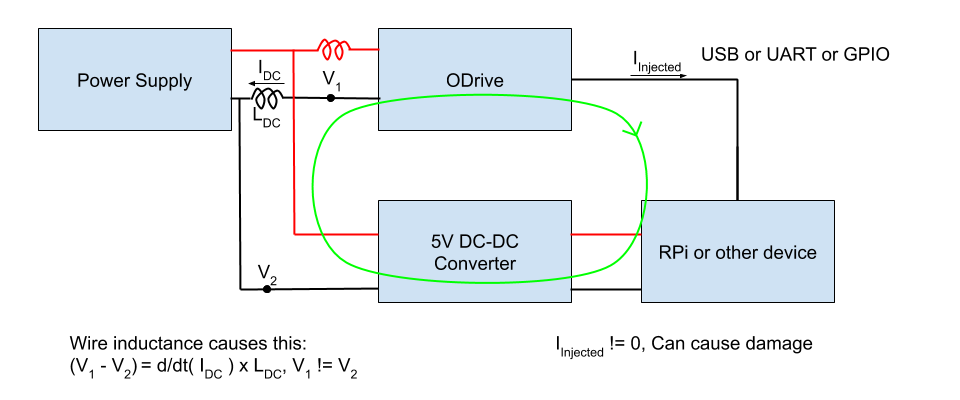
\includegraphics[width=\textwidth]{contents/figures/ground_loop_bad.png}
    \caption{Ground loop causes current flow $I_{Injected}$.}
    \label{ground_loop_bad}
    \end{figure}
    
    The issue is the inductance of the power wires between the motor controllers and the battery. This inductance, coupled with the high current drawn by the motor controllers, causes $V_1$ to be different as $V_2$, leading to potential mismatch in the voltage levels. As the motor controllers demand substantial current, the wire inductance can generate significant voltage drops along the power lines. If the voltage caused by the wire inductance and current is high enough, the 0-5V GPIO signals can swing much higher or lower than the defined voltage range, potentially exceeding safe operational limits. These fluctuations in voltage can introduce erratic behavior in the control system, compromising the performance and reliability of the motor controllers. This causes a current to flow through the ODrives GPIO pins, which can lead to unintended electrical noise and potential damage to sensitive electronic components.

    \clearpage
    \subsection{Reducing length of high-current wires}
    
    To mitigate these effects, it is substantial to keep the main powers as short as possible. All wires have some amount of inductance, which is an inherent property of any conductor through which current flows. The inductance is proportional to the length of the wires and the area of the loop formed by the power wires, meaning longer wires and larger loops will have higher inductance. This inductance can create unwanted resistance to changes in current flow, leading to voltage drops and potential interference with the system's performance. It is beneficial to keep those wires as short as possible and as close together as possible. By doing so, the loop area is minimized, and the inductance is reduced, thereby mitigating the adverse effects. However, this reduces the effect of the problem but does not eliminate it entirely, as even minimal inductance can cause issues in high-frequency and high-current applications.
    
    \subsection{Galvanic isolation}
    
    To completely minimize the possibility of creating ground loops by accident, the loop must be broken. This can be achieved by isolating the power supplies (no common ground) and connecting a dedicated signal ground between the logic and power electronics. An example of this is a single motor controller connected to a battery and a device like a Raspberry Pi connected to a different battery. It is possible to achieve the same functionality with a DC/DC isolator as shown in figure \ref{ground_loop_fix}.
    
    \begin{figure}[h]
    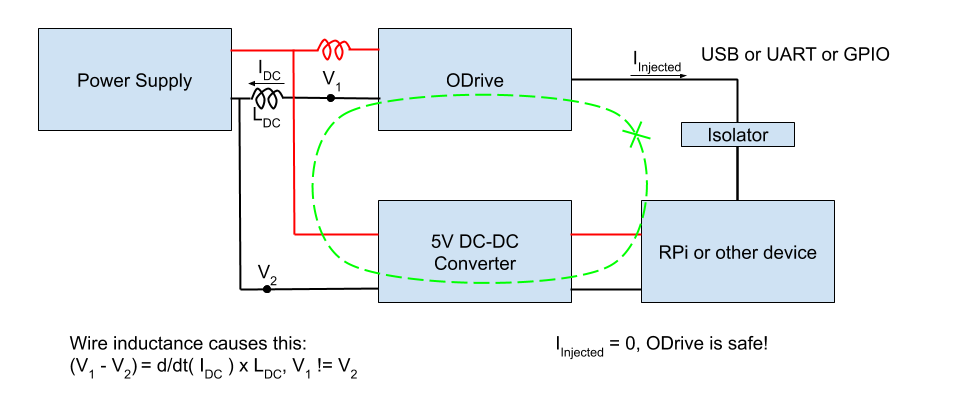
\includegraphics[width=\textwidth]{contents/figures/ground_loop_fix.png}
    \caption{Mismatched voltage levels wont introduce unwanted current flows.}
    \label{ground_loop_fix}
    \end{figure}

    \clearpage
    \subsection{Basic structure}

    

    



\section{Energy Storage}

\section{Emergency Stop}

\section{Power Distribution}

\section{Power Conversion}

\section{Power Consuming Circuits}

\section{Unused Circuits}

\section{Circuit Table}

\section{Appendix}

\paragraph{Safety Requirements}

\begin{enumerate}
    \item The rover must not include any flammable, environmentally damaging, or otherwise hazardous liquids or gasses, except:
    \begin{enumerate}
        \item Within a permanently sealed component such as a battery;
        \item Commercially-available lubricants as required by mechanical assemblies, where care is taken to avoid overuse and contamination.
    \end{enumerate}
    \item Each rover must be equipped with at least one kill switch:
    \begin{enumerate}
        \item The pressable area of the kill switch must be at least $10 cm^2$ and red in color. Levers or toggle switches are not acceptable.
        \item No other button on the rover may be red.
        \item Kill switches must be mounted on the top of the rover, with the button oriented toward the sky in the rover’s normal driving orientation.
        \item A keep out region must be maintained around the kill switch with a radius of 15cm: No components taller than the base of the kill switch may intrude on the keep out region.
        \item Kill switches must not be obstructed by a cover or sleeve which extends above the pressable surface, and must be mounted such that it will not be obstructed by other components during rover operation.
        \item The circuit including the kill switch must include appropriate circuit protection, and the “break” or “disconnect” current rating of the kill switch must exceed the current rating of the circuit protection.
        \item The function of the kill switch must not depend on the integrity of any power source or computerized system. Indirect switching by relays or similar devices is permitted as long as these are driven by the kill switch, and reliably turn off when their control line is disconnected.
        \item The function of the kill switch must not depend on the integrity of any particular wiring connection; for example, physically tearing the kill switch off the rover should produce the same effect as pressing it.
        \item If multiple kill switches are installed on the rover, pressing any one must cut all power to to the rover.
        \item The function of the kill switch must not be disabled or bypassed by any means.
        \item Rovers should have a remote motion stop for disabling a run-away rover, such as a dead man’s switch on a lead, or a radio-frequency system that operates independently of the rover communications system.
    \end{enumerate}
    
\end{enumerate}




